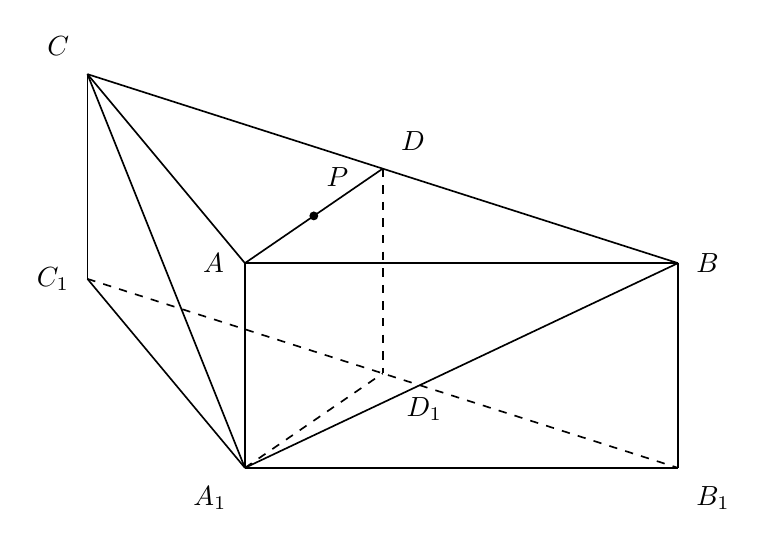
\begin{tikzpicture}[x=1cm,y=1cm,line width=.6pt,font=\normalsize]
\coordinate (C) at (0,5);
\coordinate (A) at (2,2.6);
\coordinate (B) at (7.5,2.6);
\coordinate (D) at (3.75,3.8);
\coordinate (P) at (2.8750000000,3.2000000000);
\coordinate (C1) at (0.0000000000,2.4000000000);
\coordinate (A1) at (2,0);
\coordinate (B1) at (7.5,0);
\coordinate (D1) at (3.7500000000,1.2000000000);
% top base ABC
\draw (C) -- (D) -- (B);
\draw (C) -- (A);
\draw (A) -- (B);
\draw (A) -- (D);
% lateral edges
\draw (C) -- (C1);
\draw (A) -- (A1);
\draw (B) -- (B1);
% bottom base A1B1C1
\draw (A1) -- (B1);
\draw (A1) -- (C1);
\draw[dashed] (C1) -- (B1);
% mid segment DD1
\draw[dashed] (D) -- (D1);
% auxiliary diagonals present in original
\draw (C) -- (A1);
\draw (A1) -- (B);
\draw[dashed] (A1) -- (D1);
% point P
\fill (P) circle (1.6pt);
% labels with clearance
\node[above left=3pt] at (C) {$C$};
\node[left=4pt] at (A) {$A$};
\node[right=3pt] at (B) {$B$};
\node[above right=3pt] at (D) {$D$};
\node[above right=2pt,xshift=-1pt,yshift=5pt] at (P) {$P$};
\node[left=3pt] at (C1) {$C_{1}$};
\node[below left=3pt] at (A1) {$A_{1}$};
\node[below right=3pt] at (B1) {$B_{1}$};
\node[below right=2pt,xshift=3pt,yshift=-3pt] at (D1) {$D_{1}$};
\end{tikzpicture}
